\documentclass{article}

\usepackage{graphicx}
\usepackage{tikz}
\usepackage{tikzsymbols}
\usetikzlibrary{calc,patterns,shapes.geometric}
\pagestyle{empty}
\usepackage[margin=0pt]{geometry}
\geometry{papersize={14in,12in}}

\def\centerarc[#1](#2)(#3:#4:#5){\draw[#1] ($(#2)+({#5*cos(#3)},{#5*sin(#3)})$) arc (#3:#4:#5);}

\begin{document}
	\begin{figure}
		\centering
		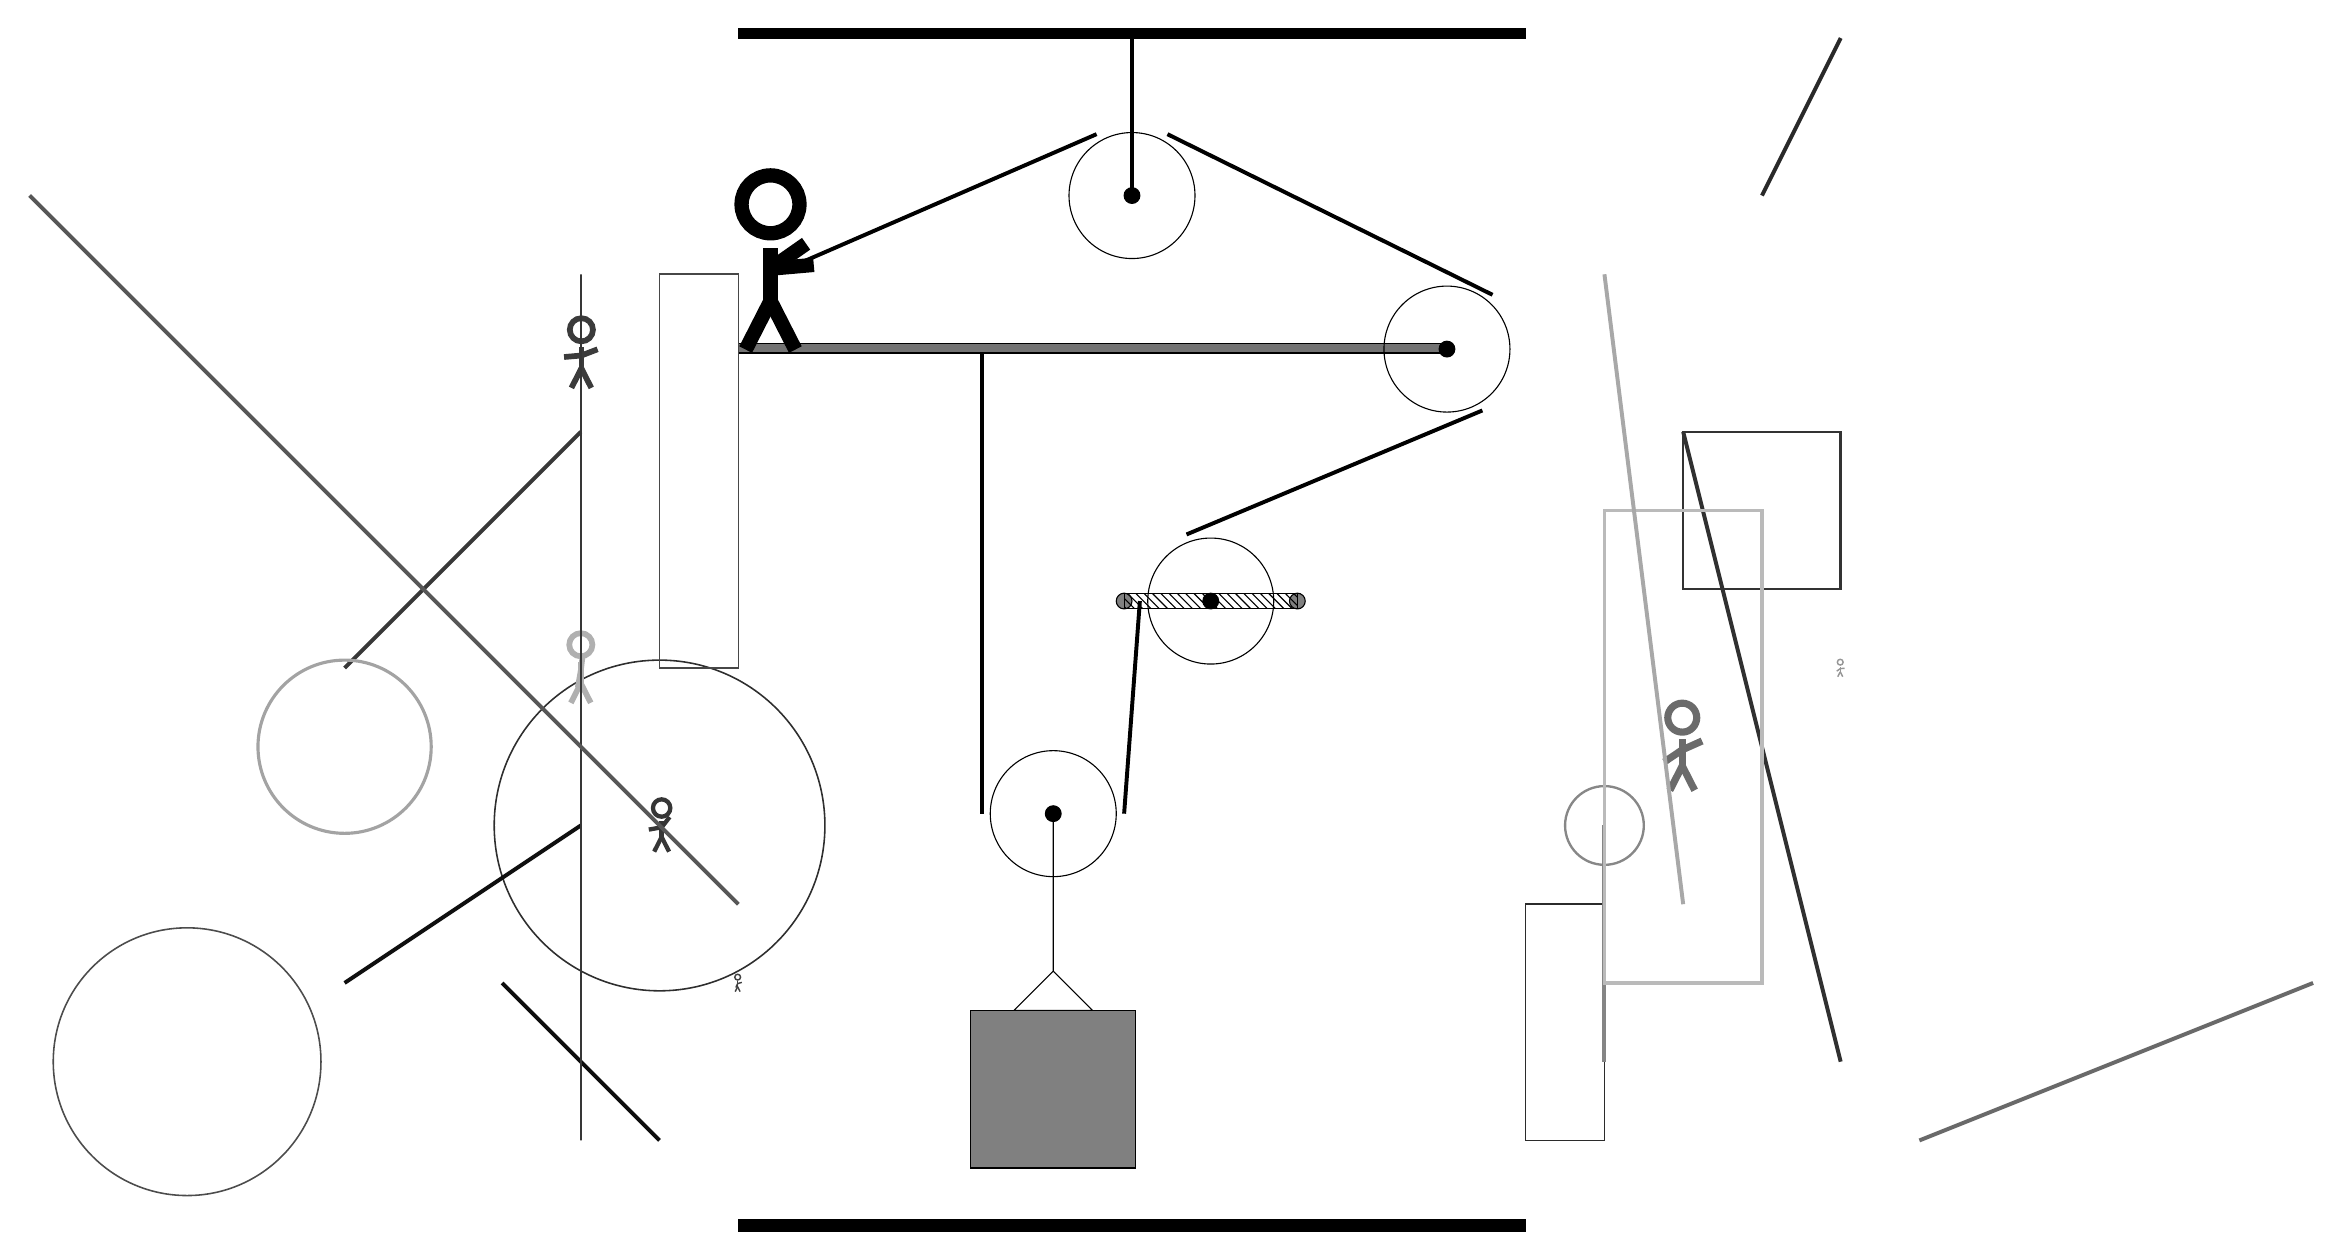
\begin{tikzpicture}
			%%%%% START %%%%%
			
			\draw[fill=black] (-2, 13) rectangle (8, 13.125);
			
			\draw[fill=black!55] (-2, 9) rectangle (7, 9.125);
			
			\draw (2, 3.15) circle (0.8);
			\draw[fill=black] (2, 3.15) circle (0.1);
			
			\draw (7, 9.05) circle (0.8);
			\draw[fill=black] (7, 9.05) circle (0.1);
			
			\draw[line width=0.5mm, color=black!81](10, 8) -- (12, 0);
			
			\draw [line width=0.2mm, color=black!70](-9, 0) circle (1.7);
			\node[line width=0.2mm, color=black!58] at (10, 4) {\Strichmaxerl[5][34][24]};
			\draw[line width=0.5mm, color=black!95](-3, -1) -- (-5, 1);
			\draw [line width=0.2mm, color=black!82](-3, 3) circle (2.1);
			\draw[line width=0.3mm, color=black!80] (10, 8) rectangle (12, 6);
			\draw[line width=0.2mm, color=black!83] (9, 2) rectangle (8, -1);
			
			\draw [line width=0.3mm, color=black!47](9, 3) circle (0.5);
			\draw[line width=0.5mm, color=black!48](9, 0) -- (9, 3);
			
			\draw[line width=0.5mm, color=black!84](12, 13) -- (11, 11);
			
			\node[line width=0.5mm, color=black!79] at (-3, 3) {\Strichmaxerl[3][10][52]};
			\node[line width=0.2mm, color=black!41] at (12, 5) {\Strichmaxerl[1][36][4]};
			\draw[line width=0.5mm, color=black!59](13, -1) -- (18, 1);
			
			\node[line width=0.5mm, color=black!31] at (-4, 5) {\Strichmaxerl[4][80][83]};
			\draw[line width=0.5mm, color=black!78](-4, 8) -- (-7, 5);
			\draw[line width=0.4mm, color=black!27] (9, 1) rectangle (11, 7);
			
			\draw [line width=0.4mm, color=black!36](-7, 4) circle (1.1);
			
			\draw[line width=0.5mm, color=black!94](-7, 1) -- (-4, 3);
			\node[line width=0.3mm, color=black!77] at (-4, 9) {\Strichmaxerl[4][5][21]};
			
			\draw[line width=0.2mm, color=black!72] (-3, 10) rectangle (-2, 5);
			\draw[line width=0.3mm, color=black!79] (-4, -1) rectangle (-4, 10);
			\node[line width=0.6mm, color=black!74] at (-2, 1) {\Strichmaxerl[1][65][16]};
			\draw[line width=0.5mm, color=black!66](-2, 2) -- (-11, 11);
			\draw[line width=0.5mm, color=black!34](9, 10) -- (10, 2);
			
			\draw[fill=white](4, 5.85) circle (0.8);
			\draw[fill=black] (4, 5.85) circle (0.1);
			\draw[fill=black!50] (2.9, 5.85) circle (0.1);
			\draw[fill=black!50] (5.1, 5.85) circle (0.1);
			\draw[pattern=north west lines, pattern color=black] (2.9, 5.95) rectangle (5.1, 5.75);
			
			\draw (3, 11) circle (0.8);
			\draw[fill=black] (3, 11) circle (0.1);
			\draw[line width=0.5mm] (3, 11) -- (3, 13);
			
			\draw (2, 3.15) -- (2, 1.15) -- (1.5, 0.65) -- (2.5, 0.65) -- (2, 1.15);
			\draw[fill=black!50] (0.95, 0.65) rectangle (3.05, -1.35);
			
			\draw[line width=0.5mm] (1.1, 9) -- (1.1, 3.15);
			\centerarc[line width=0.5mm](2, 3.15)(180:360:0.9);
			\draw[line width=0.5mm](2.9, 3.15) -- (3.1, 5.85);
			\centerarc[line width=0.5mm](4, 5.85)(110:180:0.9);
			\draw[line width=0.5mm](3.6922, 6.6957) -- (7.45, 8.2706);
			\centerarc[line width=0.5mm](7, 9.05)(-60:50:0.9);
			\draw[line width=0.5mm](7.5785, 9.7394) -- (3.45, 11.7794);
			\centerarc[line width=0.5mm](3, 11)(60:120:0.9);
			\draw[line width=0.5mm](2.55, 11.7794) -- (-1.2, 10.15);
			
			\node at (-1.5, 10.15) {\Strichmaxerl[10][-175][35]};
			
			\draw[fill=black] (-2, -2) rectangle (8, -2.15);
			
			%%%%% END %%%%%
		\end{tikzpicture}
	\end{figure}	
\end{document}